\section{Cel prac i wizja produktu}
\label{sec:cel-wizja}

% \emph{Charakterystyka problemu, motywacja projektu (w tym przegląd
  % istniejących rozwiązań prowadząca do uzasadnienia celu prac), ogólna
  % wizja produktu, krótkie studium wykonalności i analiza zagrożeń.}

Od wielu wieków istnieje potrzeba ochrony tajnych informacji przed przechwyceniem przez osoby niepowołane. Znane są przykłady takich czynności pochodzące już z czasów starożytnych. Pierwszym powszechnie znanym przykładem jest szyfr Cezara, który był używany przez rzymskiego wodza do ochrony poufnej korespondencji. Innym dobrze znanym przykładem jest szyfr Enigmy, który odegrał ważną rolę podczas II wojny światowej.

Początkowo szyfrowanie było używane w nielicznych przypadkach, obecnie towarzyszy ludziom każdego dnia. Największą domeną, w której stosowana jest kryptografia jest niewątpliwie ochrona danych cyfrowych. Wykorzystywana jest m.in. do szyfrowania komunikacji, danych zapisanych na różnych nośnikach, do uwierzytelniania, jest podstawą walut elektronicznych itp.

Ze względu na postęp technologiczny, stare metody szyfrowania nie są już bezpieczne. Przykładem może być szyfr DES, który został zatwierdzony jako standard w 1976 roku. Od tamtej pory moc obliczeniowa komputerów na tyle się zwiększyła, że obecnie DES można złamać przy pomocy ataków \textit{brute force} i jest on obecnie uważany za algorytm niezapewniający odpowiedniego bezpieczeństwa.

W celu zapewnienia bezpieczeństwa stosowane współcześnie szyfry wymagają wykonania wielu operacji aby dane zaszyfrować oraz odszyfrować. W połączeniu z rosnąca popularnością kryptografii, jest to motywacją do poszukiwania wydajnych sposobów szyfrowania -- przystosowywania istniejących procesorów do szybkiego wykonywania instrukcji szyfrujących, lub nawet tworzenia osobnych szyfrujących układów sprzętowych. Ten projekt zajmuje się zagadnieniem szyfrowania AES przy pomocy układu sprzętowego zrealizowanego na platformie FPGA.

\subsection{Motywacja projektu}
Popularność sprzętowych układów projektowanych z myślą o wykonywaniu specyficznych zadań ciągle rośnie. W dzisiejszych czasach można je znaleźć w szerokiej gamie zastosowań, od analizatorów stanów logicznych (np. Saleae Logic 16 \cite{saleae-fpga}) przez wysokowydajne systemy bazodanowe (np. IBM Netezza \cite{netezza-fpga}) do wykorzystania w pojazdach kosmicznych NASA \cite{nasa-fpga}.

Również kryptografia znajduje zastosowanie w wielu dziedzinach -- szyfrowanie plików różnymi algorytmami (np. program \textit{openssl} \cite{openssl}), zapewnienie poufności komunikacji (np. protokół SSL) itd. Współczesne procesory (np. Intel, AMD) wyposażone są w zestawy instrukcji przeznaczonych do szyfrowania (AES-NI) \cite{aes-processors}. 

Główną motywacją projektu jest chęć eksploracji zagadnienia wykorzystania układów logiki programowalnej FPGA do rozwiązywania problemów dziedziny kryptografii na przykładzie algorytmu AES.

\subsection{Wizja produktu}
Celem projektu inżynierskiego jest zaimplementowanie sprzętowego układu szyfrującego algorytmem AES na platformie FPGA, oraz praktyczne zaprezentowanie jego działania. Końcowy produkt będzie umożliwiał użytkownikowi szyfrowanie i deszyfrowanie plików. Sposób szyfrowania AES będzie zgodny ze standardem FIPF-197 \cite{aes-standard} oraz produkt będzie kompatybilny z obecnie istniejącym rozwiązaniem -- programem \textit{openssl} \cite{openssl}.

Produktem końcowym będzie program konsolowy przystosowany do uruchomienia na systemach operacyjnych Ubuntu, oraz karta SD zawierająca skrypt programujący układ FPGA. Do uruchomienia produktu potrzebna będzie płytką FPGA Terasic DE1-SOC podłączona do komputera.

Płytka Terasic DE1-SOC będzie komunikować się z komputerem przez kabel USB (rys. \ref{fig:system-architecture-basic}). Protokołem komunikacji będzie UART tunelowany przez USB. Na płytce znajduje się konwerter umożliwiający konwersję USB-UART firmy FTDI. W systemach operacyjnych Ubuntu zintegrowany jest sterownik współpracujący z tym układem, który nie wymaga dodatkowej instalacji.

\begin{figure}[!h]
\centering
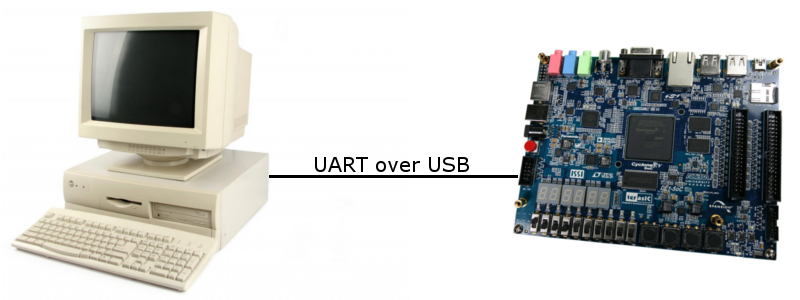
\includegraphics[width=6in]{pictures/system-architecture-basic.png}
\caption{Architektura systemu (na zdjęciu laptop Dell XPS 13 \cite{laptop} oraz płytka Terasic DE1-SOC \cite{plytka})}
\label{fig:system-architecture-basic}
\end{figure}

W celu zaszyfrowania pliku, użytkownik komputera będzie musiał uruchomić skrypt będący częścią produktu, który będzie odczytywał z dysku kolejne bloki danych w postaci jawnej, wysyłał je do układu FPGA oraz odbierał bloki danych zaszyfrowanych i zapisywał je do innego pliku. Układ FPGA będzie odbierał bloki danych, szyfrował oraz je odsyłał w postaci zaszyfrowanej. Deszyfrowanie będzie przebiegać analogicznie. Szyfrowanie plików większych niż 128b będzie przebiegać w trybie wiązania bloków CBC. Ze względu na możliwość wystąpienia błędów podczas komunikacji UART, zaimplementowana zostanie obsługa błędów oparta o sumę kontrolną CRC16.

Programowanie układu FPGA będzie zrealizowanie w sposób nie wymagający od użytkownika wiedzy technicznej -- będzie wykonywane automatycznie przy starcie płytki FPGA. Włączenie płytki w taki sposób aby układ FPGA został odpowiednio zaprogramowany będzie wymagało jedynie przestawiania kilku przełączników oraz włożenia dostarczonej karty SD do czytnika. 

\subsection{Studium wykonalności}
Szyfrowanie AES jest dobrze znanym i udokumentowanym algorytmem, dla którego istnieje wiele implementacji. Również FPGA jest technologią, która istnieje na rynku od wielu lat oraz znajduje zastosowanie w różnych dziedzinach. 

Jednoosobowy zespół projektowy miał już okazję implementować projekt o podobnej złożoności w ramach zajęć z przedmiotu \textit{Technika Mikroprocesorowa 2}. To w połączeniu ze wstępną analizą dziedziny projektu oraz dostępnych źródeł pozwala stwierdzić, że projekt jest wykonalny w ramach dostępnych zasobów ludzkich, technologicznych oraz czasowych.

\subsection{Analiza ryzyka}
Proces tworzenia produktu wiąże się z wieloma zagrożeniami. W fazie planowania projektu została przeprowadzona analiza ryzyka wraz z planowaniem reakcji na zaistniałe utrudnienia.

\begin{enumerate}
\item Zbyt mała liczba jednostek logicznych w układzie FPGA. Moduły szyfrowania i deszyfrowania AES mogą się okazać zbyt złożone, aby mogły się zmieścić w wybranym układzie FPGA. W takim przypadku w celu zmniejszenia złożoności projektu można będzie podjąć następujące kroki:
	\begin{itemize}
	\item zmniejszenie długości klucza szyfrowania
	\item zmiana projektu modułów szyfrujących i deszyfrujących -- zastosowanie przetwarzania synchronicznego, w którym rundy szyfrowania wykonywane są w kolejnych cyklach zegara przez ten sam fragment układu
	\item dostarczenie dwóch osobnych produktów - szyfrującego i deszyfrującego
	\end{itemize}
\item Brak możliwości użycia układu UART znajdującego się na płytce, co może prowadzić do konieczności wykorzystania osobnego konwertera USB-UART. Spowodowałoby to utrudnienia dla użytkownika końcowego związane z potrzebą użycia zewnętrznego konwertera. W przypadku wystąpienia takiego scenariusza wszystkie konieczne do wykonania czynności zostaną dokładnie opisane w dokumentacji użytkownika.
\item Brak możliwości uruchomienia płytki w taki sposób, aby układ FPGA został automatycznie zaprogramowany przy starcie. Prowadziłoby to do utrudnienia dla użytkownika końcowego związanego z koniecznością ręcznego programowania płytki. W przypadku wystąpienia takiego scenariusza wszystkie konieczne do wykonania czynności zostaną dokładnie opisane w dokumentacji użytkownika.
\item Problemy związane z niezerowym czasem propagacji sygnału oraz innymi właściwościami fizycznymi układu FPGA, powodującymi niedeterministyczne oraz trudne do wykrycia błędy. Aby temu zapobiec w projekcie zostaną skonfigurowane ograniczenia czasowe (ang. \textit{timing constraints}).
\item Czynniki losowe opóźniające pracę lub uniemożliwiające ukończenie projektu na czas, np. choroba. W celu minimalizacji skutków takich sytuacji w harmonogramie prac zostanie przewidziany czas przeznaczony na nadrobienie zaległości.
\item Uszkodzenie sprzętu ze względu na wadę produkcyjną lub niekompetencję zespołu projektowego.
\end{enumerate}


\newpage